\begin{frame}[noframenumbering,plain]
    \setcounter{framenumber}{1}
    \maketitle
\end{frame}
\note{
    Приветствие.
    Презентация расчитана на 20 минут.

    Удачи.
}


\begin{frame}
    \frametitle{Мотивация}
    Интерес обусловлен важностью для многих
    инженерных применений, связанных с высокими температурами: оценки
    эффективности систем охлаждения, моделирования теплопередачи в деталях
    газотурбинных двигателей, космической техники, летательных аппаратов,
    контроль тепловых процессов при производстве стекла и др.

%    \includegraphics[width=3.cm,height=2.5cm]{ex1}
    \hfill
%    \includegraphics[width=3cm,height=2.5cm]{ex2}
    \hfill
%    \includegraphics[width=3cm,height=2.5cm]{ex4}
    \begin{itemize}
        \item Теоретическое исследование моделей сложного теплообмена с
        полным уравнением переноса излучения
        (\textit{А. А. Амосов, C. T. Kelley, M. Laitinen, T. Tiihonen, P.-E. Druet и др.})
        \item Однозначная разрешимость различных задач радиационно-кондуктивного теплообмена
        (\textit{F. Asllanaj, M. Ghattassi, M. Porzio, M. Thompson и др.})
        \item Анализ квазистационарных моделей сложного теплообмена на основе $SP_1$ и $SP_3$-приближений
        (\textit{R. Pinnau, O. Tse})
        \item Однозначная разрешимость краевых задач для моделей сложного теплообмена
        (\textit{А. Ю. Чеботарев, А. Е. Ковтанюк, Г. В. Гренкин})
        \item Теоретический анализ обратных задач для моделей тепломассопереноса
        (\textit{С. Г. Пятков, О.М. Алифанов, и др.})
    \end{itemize}
\end{frame}
\note{
    \begin{itemize}
        \item Интерес к моделированию ...
        \item Отметим работы ...
        \item Однако, существенная часть проблем с анализом моделей, разработкой ...
    \end{itemize}
}

\subsection{Граничная обратная задача}\label{subsec:rev}
\begin{frame}
    \textbf{Модель сложного теплообмена} в $P_1$ приближении
    имеет следующий вид
    \begin{wrapfigure}{r}{0.5\textwidth}
        \centering{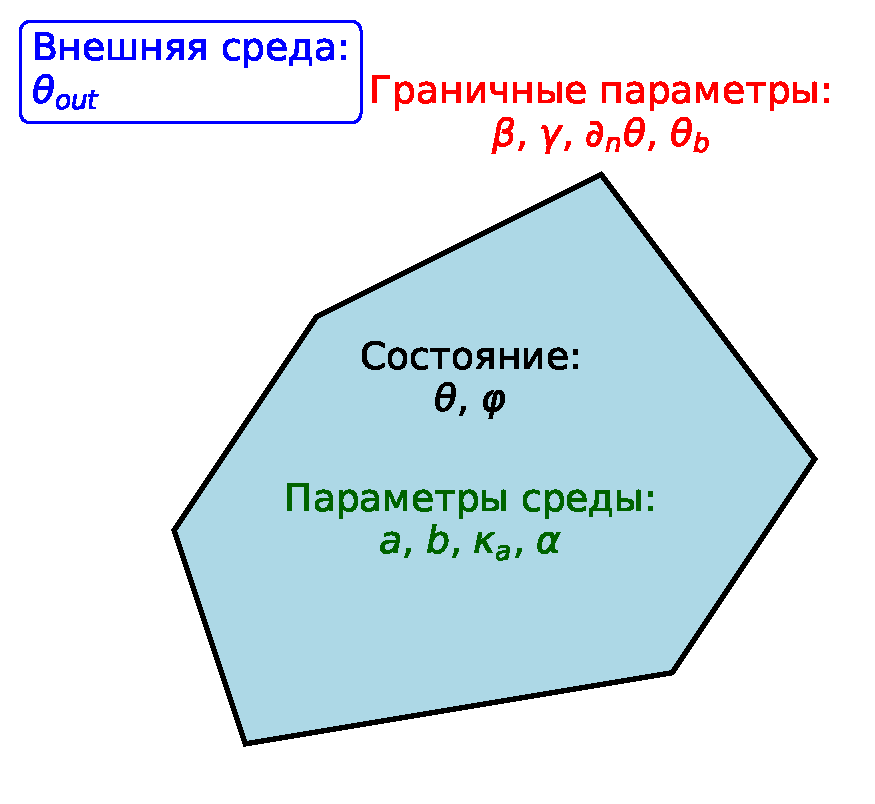
\includegraphics[width=1\linewidth]{model}}
    \end{wrapfigure}
    \begin{gather*}
        - a \Delta \theta + b \kappa_a(\theta ^ 3 | \theta | - \varphi) = 0, \\
        - \alpha \Delta \varphi + \kappa_a (\varphi - \theta ^3 | \theta |) = 0.
    \end{gather*}

    Система двух эллиптических уравнений дополняется следующими краевыми условиями
    \begin{equation*}
        \begin{aligned}
            a \partial_n \theta + \beta (\theta - \theta _b) = 0, \\
            \alpha \partial_n \varphi + \gamma(\varphi - \theta_b ^4 ) = 0.
        \end{aligned}
    \end{equation*}

    Функции $\gamma, \theta_b, \beta$ известны.

    \textbf{Обратная задача} заключается в отыскании тройки $\theta, \varphi, u$
    по некоторому дополнительному условию.
    Здесь $u$ - неизвестный параметр среды (\textit{управление}).\\
    \textbf{Задача с условиями Коши} заключается в отыскании \textit{состояния}
    по информации о температуре на границе и тепловому потоку.

\end{frame}
\note{
    \begin{itemize}
        \item Центральным местом работы является модель сложного теплообмена, которая приведена на слайде
        \item Доказательство однозначной разрешимости было получено Александром Юрьевичем в 2015 году.
        \item Обратная задача ставится в том случае, если неизвестны параметры среды, но граничные условия
        дополняются дополнительным условием, которое называется условие переопределения.
        \item Сходные с ними задачи, с данными Коши возникают в том случае\ldots (терминология М.\ М.\ Лаврентьева)
        \item Обратные задачи актуальны в том ключе, что часто в рамках производственного процесса мы должны
        контролировать поле температур
        (охлаждение стекла и металлов, изготовление полимеров) - не можем менять сам материал,
        но можем менять внешние условия (меняя граничные параметры).
        Различные инженерные установки, газотурбинные двигатели, летательные аппараты
        - их материалы предопределены конструкторскими задачами,
        но различные покрытия могут служить важным инструментом в управлении температурным полем.

        \item $\theta, \varphi$ -- состояние, $u$ -- управление (неизвестный параметр среды)

    \end{itemize}
}

\begin{frame}
    \frametitle{Цели и задачи работы}
    \textit{Целью работы} является разработка математических
    и численных методов решения обратных задач сложного теплообмена.
    Это включает в себя как теоретическое обоснование,
    так и разработку алгоритмов и программных комплексов,
    которые позволяют эффективно решать рассматриваемые задачи.
    \begin{itemize}
        \item исследование корректности моделей процессов сложного теплообмена,
        описываемых краевыми и начально-краевыми задачами для нелинейных
        квазистационарных и квазилинейных уравнений;
        \item разработка оптимизационных алгоритмов решения обратных задач и
        задач с краевыми условиями Коши, теоретический анализ и обоснование их сходимости;
        \item разработка комплекса программ для проведения вычислительных
        экспериментов и тестирования предложенных алгоритмов.
        \item Анализ свойств устойчивости и стабилизации
        процессов сложного теплообмена методами численного моделирования.
    \end{itemize}
\end{frame}
\note{
    \begin{itemize}
        \item В работе рассматриваются диффузионные модели сложного теплообмена
        в рамках так называемого $Р_1$ приближения уравнения переноса излучения,
        где функция, описывающая тепловое излучение является интенсивностью излучения,
        усредненной по всем направлениям.
        \item Обратные задачи возникают в случае ...
        \item
        \item \textbf{Целью работы} является разработка математических и численных методов решения...
        \begin{itemize}
            \item Теоретическое исследование квазистационарных и квазилинейных моделей
            \item Сведение обратных задач к задачам оптимального управления.
            \item Доказательство сходимости задач оптимального управления к начальным постановкам
            \item Программная реализация предложенных методов решения и апробация иъ эффективности.
        \end{itemize}
    \end{itemize}
}
